% DISTANCE ON THE COORDINATE PLANE - WORKSHEET 0 (IN-CLASS INSTRUCTION)
\documentclass[12pt, letterpaper, fleqn]{article}

% ----------------------------------------------------------
% PACKAGES
% ----------------------------------------------------------
\usepackage{graphicx}
\usepackage{xcolor}
\usepackage[most]{tcolorbox}
\usepackage{amsmath, amssymb}
\usepackage{fancyhdr}
\usepackage[utf8]{inputenc}
\usepackage[T1]{fontenc}
\usepackage{enumitem}
\usepackage{geometry}
\usepackage{tikz}
\usepackage{needspace}
\usepackage{multicol}

\usetikzlibrary{arrows.meta, calc, positioning}

% ----------------------------------------------------------
% PAGE SETUP
% ----------------------------------------------------------
\usepackage{times}
\geometry{letterpaper, top=1.25in, bottom=1.25in, marginpar=0.5in}

% ----------------------------------------------------------
% HEADER / FOOTER
% ----------------------------------------------------------
\newcommand{\logowidth}{3cm}
\setlength{\headheight}{20pt}
\setlength{\footskip}{40pt}

\pagestyle{fancy}
\fancyhf{}
\fancyhead[C]{\small\bfseries Distance on the Coordinate Plane}
\fancyfoot[L]{\raisebox{2pt}{
\includegraphics[width=\logowidth]{../kss.png}}}
\fancyfoot[C]{\thepage}
\fancyfoot[R]{8.23.0}

\renewcommand{\footrulewidth}{0.2pt}

% ----------------------------------------------------------
% THEME COLOR
% ----------------------------------------------------------
\definecolor{customteal}{HTML}{2fbdb9}

% ----------------------------------------------------------
% HELPER MACROS
% ----------------------------------------------------------
\newcommand{\blank}{\underline{\hspace{2.2cm}}}
\newcommand{\blanklong}{\underline{\hspace{6.5cm}}}
\newcommand{\blankshorter}{\underline{\hspace{1.5cm}}}

% ----------------------------------------------------------
% DOCUMENT
% ----------------------------------------------------------
\begin{document}

\textbf{Name:} \underline{\hspace{5cm}}
\hfill
\textbf{Date:} \underline{\hspace{3cm}}\\

% ==========================================================
% SECTION 1: FOUNDATION
% ==========================================================
\begin{tcolorbox}[colback=customteal!20]
    \large\textcolor{black}{\textbf{Foundation: Using Pythagorean Theorem on a Grid}}
\end{tcolorbox}

\vspace{3mm}

\noindent
To find the distance between any two points on a coordinate plane, you don't need a special new formula! You can just use the \textbf{Pythagorean Theorem} ($a^2 + b^2 = c^2$).

\begin{itemize}
    \item \textbf{The Hypotenuse ($c$):} The diagonal line connecting the two points is the hypotenuse of an invisible right triangle.
    \item \textbf{The Legs ($a$ and $b$):} You can find the lengths of the legs by drawing horizontal and vertical lines to connect the two points. The length of the legs is just the difference in the $x$-values and $y$-values!
\end{itemize}

\vspace{4mm}

% ==========================================================
% VISUAL REPRESENTATION
% ==========================================================
\begin{tcolorbox}[colback=white, colframe=black!25, boxrule=0.6pt, arc=4mm, left=6mm, right=6mm, top=5mm, bottom=5mm]

\textbf{Visual Representation: Drawing the Triangle}

\medskip

\begin{center}
\begin{tikzpicture}[scale=0.8]
% Grid
\draw[step=1cm,gray!30,very thin] (-1,-1) grid (6,5);
\draw[thick,->] (-1.5,0) -- (6.5,0) node[right] {$x$};
\draw[thick,->] (0,-1.5) -- (0,5.5) node[above] {$y$};

% Points
\filldraw[black] (1,1) circle (3pt) node[below left] {$A(1,1)$};
\filldraw[black] (4,5) circle (3pt) node[above right] {$B(4,5)$};

% Hypotenuse
\draw[thick, blue] (1,1) -- (4,5) node[midway, above left] {$c$};

% Legs
\draw[dashed, red, thick] (1,1) -- (4,1) node[midway, below] {$a = 3$};
\draw[dashed, green!60!black, thick] (4,1) -- (4,5) node[midway, right] {$b = 4$};

% Right angle
\draw (3.7, 1) -- (3.7, 1.3) -- (4, 1.3);

\end{tikzpicture}
\end{center}

\medskip
\begin{itemize}
    \item The horizontal distance ($a$) from $x=1$ to $x=4$ is $3$.
    \item The vertical distance ($b$) from $y=1$ to $y=5$ is $4$.
    \item Now use the theorem: $3^2 + 4^2 = c^2 \implies 9 + 16 = 25 \implies c = \sqrt{25} = 5$.
    \item The distance from $A$ to $B$ is exactly $5$ units.
\end{itemize}

\end{tcolorbox}

\vspace{4mm}

\newpage

% ==========================================================
% WORKED EXAMPLES
% ==========================================================
\begin{tcolorbox}[colback=customteal!20]
\large\textcolor{black}{\textbf{Finding Distance Without a Grid}}
\end{tcolorbox}

\noindent
You don't always have to draw a picture. You can calculate the lengths of the legs mathematically by subtracting the coordinates.

\vspace{3mm}

\begin{tcolorbox}[colback=white, colframe=black!25, boxrule=0.6pt, arc=4mm, left=6mm, right=6mm, top=5mm, bottom=5mm]

\textbf{Worked Example 1: Calculating Distance}

\medskip

\textbf{Problem:} Find the exact distance between $(-3, 2)$ and $(5, -4)$.

\medskip

\textbf{Solution:}
\begin{itemize}
    \item \textbf{Step 1 (Find Horizontal Leg $a$):} Subtract the $x$-values. 
    \[ 5 - (-3) = 8 \]
    \item \textbf{Step 2 (Find Vertical Leg $b$):} Subtract the $y$-values.
    \[ 2 - (-4) = 6 \]
    \item \textbf{Step 3 (Use Pythagorean Theorem):}
    \begin{align*}
        a^2 + b^2 &= c^2 \\
        8^2 + 6^2 &= c^2 \\
        64 + 36 &= c^2 \\
        100 &= c^2
    \end{align*}
    \item \textbf{Step 4 (Square Root):} $\sqrt{100} = 10$. The distance is $10$ units.
\end{itemize}

\end{tcolorbox}

\vspace{4mm}

% ==========================================================
% PRACTICE 1
% ==========================================================
\begin{tcolorbox}[colback=white!15, colframe=black, boxrule=1.5pt, arc=4mm, left=6mm, right=6mm, top=5mm, bottom=5mm]

\textbf{Guided Practice: Basic Operations}

\medskip

\noindent
\textbf{1.} Find the distance between $(0, 0)$ and $(5, 12)$.
\vspace{2cm}

\noindent
\textbf{2.} Plot the points $(-2, 1)$ and $(2, 4)$ on a piece of graph paper. Draw the right triangle. What are the lengths of the legs? What is the hypotenuse?
\vspace{2.5cm}

\end{tcolorbox}

\newpage

% ==========================================================
% THINKING PROBLEM
% ==========================================================
\begin{tcolorbox}[colback=customteal!20]
\large\textcolor{black}{\textbf{Deeper Thinking: Applications on the Grid}}
\end{tcolorbox}

\vspace{3mm}

\begin{tcolorbox}[colback=white!15, colframe=black, boxrule=1.5pt, arc=4mm, left=6mm, right=6mm, top=5mm, bottom=5mm]

\textbf{Deeper Thinking Problem 1: The Triangle Perimeter}

\medskip

\noindent
A triangle is drawn on a coordinate plane with vertices at:
\[ A(-4, -1), \ B(2, -1), \ C(-1, 3) \]

\vspace{5mm}

\noindent
\textbf{a)} First, find the length of side $AB$. Notice that this side is perfectly horizontal, so you don't even need the Pythagorean Theorem. What is the distance?

\vspace{2cm}

\noindent
\textbf{b)} Now, find the length of side $BC$. This is a diagonal, so use the Pythagorean theorem. Find the horizontal and vertical distance from $B$ to $C$ first. 

\vspace{3cm}

\noindent
\textbf{c)} Next, find the length of side $AC$. 

\vspace{3cm}

\noindent
\textbf{d)} Add up all three sides to find the perimeter of Triangle $ABC$. 

\vspace{2cm}

\end{tcolorbox}

\end{document}
